\documentclass{article}

\usepackage{neurips_2024}

\usepackage[utf8]{inputenc}
\usepackage[T1]{fontenc}
\usepackage{hyperref}
\usepackage{url}
\usepackage{booktabs}
\usepackage{amsfonts}
\usepackage{amsmath}
\usepackage{amssymb}
\usepackage{amsthm}
\usepackage{nicefrac}
\usepackage{microtype}
\usepackage{xcolor}
\usepackage{algorithm}
\usepackage{algorithmic}
\usepackage{graphicx}
\usepackage{multirow}
\usepackage{subcaption}
\usepackage{bm}
\usepackage{enumitem}
\usepackage{wrapfig}
\usepackage{thmtools}

\newtheorem{theorem}{Theorem}
\newtheorem{lemma}[theorem]{Lemma}
\newtheorem{proposition}[theorem]{Proposition}
\newtheorem{corollary}[theorem]{Corollary}
\newtheorem{remark}{Remark}
\newtheorem{definition}{Definition}
\newtheorem{assumption}{Assumption}

\newcommand{\erank}{\mathrm{erank}}
\newcommand{\srank}{\mathrm{srank}}
\newcommand{\tr}{\mathrm{tr}}
\newcommand{\diag}{\mathrm{diag}}
\newcommand{\RR}{\mathbb{R}}
\newcommand{\EE}{\mathbb{E}}
\newcommand{\cL}{\mathcal{L}}
\newcommand{\cT}{\mathcal{T}}
\newcommand{\cW}{\mathcal{W}}
\newcommand{\cH}{\mathcal{H}}
\newcommand{\cS}{\mathcal{S}}
\newcommand{\cN}{\mathcal{N}}
\newcommand{\cO}{\mathcal{O}}

\title{Can the Optimizer Prevent Loss of Plasticity? \\ Second-Order Methods Meet Spectral Diversity Preservation}

\author{%
  Anonymous Author(s) \\
  \texttt{anonymous@institution.edu}
}

\raggedbottom
\begin{document}

\maketitle

\begin{abstract}
Neural networks trained on non-stationary data streams progressively lose their ability to learn new tasks, a phenomenon known as loss of plasticity (LoP). While existing solutions predominantly target architecture or explicit regularization, the role of the optimizer itself remains underexplored. In this paper, we investigate whether second-order opitmizers can inherently mitigate LoP. We uncover a nuanced answer governed by two factors: \emph{network depth} and \emph{normalization structure}. We prove that both Natural Gradient Descent and Hessian-based methods equalize per-direction convergence rates and provide quantifiable amplification over SGD for near-frozen and cloned units. Yet this advantage does not hold uniformly: in deep batch-normalized networks, second-order methods maintain plasticity but overfit via sharp-minima convergence; in shallow networks without BN, outlier eigenvalues degrade preconditioning, paradoxically accelerating rank collapse. To address both failure modes, we propose two complementary mechanisms: CWN (Centered Weight Normalization) integrated directly into K-FAC to replicate BN's plasticity-preserving properties without architecture modification, and SDP (Spectral Diversity Preservation), a lightweight rescaling of weight's singular values acitng as a spectral analog of BN. Across six second-order optimizers and four continual-learning benchmarks, our methods consistently achieve near-zero dormant units and highest stable ranks, matching or surpassing dedicated plasticity-preserving methods.

\end{abstract}

\section{Introduction}
\label{sec:intro}

Neural networks achieve remarkable performance in stationary settings, yet exhibit a 
troubling degradation when the data distribution shifts over time. In continual 
learning, reinforcement learning with non-stationary 
environments, and online adaptation, networks 
gradually lose their capacity to acquire new information, a phenomenon termed \emph{loss 
of plasticity} (LoP)~\citep{lyle2023understanding, dohare2024loss}. Unlike catastrophic 
forgetting, which concerns the erasure of prior knowledge, LoP 
reflects a fundamental erosion of the network's \emph{learning capacity itself}: the seminal 
work of~\citet{dohare2024loss} demonstrated that standard backpropagation with SGD 
inevitably loses plasticity on long task sequences, eventually performing no better than a 
shallow linear model. This finding has sparked a wave of research across supervised 
learning~\citep{lewandowski2025spectral, farias2025snr, shin2024dash}, reinforcement 
learning~\citep{nikishin2023plasticity, juliani2024plasticity, tang2025mitigating}, and 
multi-agent settings~\citep{qin2024reborn}.

The symptoms of LoP are well-characterized and interrelated. The fraction of \emph{dormant 
neurons} (units producing near-zero activations) increases over training~\citep{sokar2023dormant}. 
The \emph{effective rank} of weight matrices and feature representations collapses, 
reducing expressive capacity, weight magnitudes grow unboundedly saturating activation 
functions, and the generalization gap widens~\citep{dohare2024loss}. Several theoretical frameworks have 
emerged to explain these symptoms. \citet{lyle2023understanding} showed that gradient descent pushes parameters toward regions 
of the loss landscape that are increasingly hostile to new objectives, as evidenced by 
growing Hessian spectral norm and negative gradient interference over training. \citet{lewandowski2024curvature} proposed that the reduction in the rank of the Hessian 
of the training objective, which they term \emph{Hessian spectral collapse}, is a 
consistent explanation for LoP, demonstrating that this loss of curvature directions 
reliably coincides with plasticity loss across multiple factors and benchmarks. 
\citet{joudaki2026barriers} further provided a dynamical-systems formalization, proving that 
LoP arises from entrapment of gradient dynamics within \emph{invariant sub-manifolds} of 
parameter space, including frozen-unit manifolds from activation saturation and cloned-unit 
manifolds from representational redundancy, and that the very mechanisms promoting 
generalization in static settings actively steer networks into these LoP manifolds.

Current approaches to LoP predominantly modify the architecture or add explicit 
regularization atop standard first-order optimizers. Continual 
backpropagation~\citep{dohare2024loss} randomly reinitializes dormant neurons, injecting 
diversity through a non-gradient mechanism. \citet{lyle2025disentangling} showed that layer 
normalization combined with weight decay mitigates multiple independent causes of plasticity 
loss simultaneously. Other methods take a variety of forms: shrink-and-perturb~\citep{ash2020warm, 
juliani2024plasticity} periodically contracts and randomly perturbs network weights to 
escape stagnant regions; spectral regularization~\citep{lewandowski2025spectral} prevents 
rank collapse by constraining singular values; and approaches such as utility-based 
perturbation~\citep{elsayed2024upgd}, regenerative regularization~\citep{kumar2025l2init}, 
and rank-preserving weight decay~\citep{wu2026rank} each target a different proximal cause 
of plasticity loss through selective reinitialization, proximity-to-initialization 
penalties, and norm-rank decoupling, respectively. However, all these methods operate atop first-order optimizers 
(SGD, Adam), leaving a fundamental question unaddressed:

\begin{center}
\emph{Can the optimizer itself, through its use of curvature information, mitigate loss 
of plasticity?}
\end{center}

% This question is motivated by a convergence of theoretical insights:
% \begin{enumerate}[leftmargin=*,nosep]
%     \item \citet{lewandowski2024curvature}: Loss of curvature information is a root cause of LoP $\Rightarrow$ optimizers maintaining curvature awareness may resist it.
%     \item \citet{gurari2018gradient}: Gradient descent operates in a tiny subspace of the top Hessian eigenvectors $\Rightarrow$ first-order updates are inherently low-rank, driving rank collapse.
%     \item \citet{joudaki2026barriers}: First-order gradient dynamics are trapped in LoP manifolds due to the vanishing of transverse gradient components $\Rightarrow$ second-order methods, whose update geometry differs fundamentally, may escape these manifolds.
%     \item \citet{ghorbani2019investigation}: Batch normalization suppresses outlier Hessian eigenvalues $\Rightarrow$ the Hessian spectral structure mediates whether second-order methods can leverage curvature effectively.
% \end{enumerate}

% \paragraph{Key observations.}
% Through systematic experiments across architectures, we identify a depth-dependent 
% dichotomy. In shallow networks without BatchNorm, second-order methods fail to maintain 
% plasticity: large Hessian outliers~\citep{ghorbani2019investigation} corrupt 
% preconditioning, effectively reducing second-order updates to poorly-scaled first-order 
% ones. In deeper networks with BatchNorm, second-order optimizers automatically preserve 
% plasticity but suffer from overfitting due to rapid convergence to sharp 
% minima~\citep{shin2025sassha}. These observations motivate both our theoretical analysis 
% and our proposed remedies.

\paragraph{Contributions.} We make the following contributions:
\begin{enumerate}[leftmargin=*,nosep]
    \item \textbf{Can second-order optimizers intrinsically mitigate LoP?}
    (Section~\ref{sec:theory}): We examine two structural factors, network depth and 
    normalization architecture, and show that second-order optimizers can automatically 
    counteract LoP when the Hessian (or Fisher) is well-conditioned. We prove that 
    preconditioned updates preserve spectral diversity in weight matrices, establish 
    per-layer weight norm contraction, and show that K-FAC further equalizes the condition 
    ratio and amplifies gradient signals for near-frozen and near-cloned units.

    \item \textbf{Spectral Diversity Preservation for Hessian-based optimizers}
    (Section~\ref{sec:method}): When BatchNorm is present, we propose SDP, a geometric 
    mean interpolation on weight singular values applied at task boundaries that provably 
    reduces the condition number while preserving singular subspaces. We further formalize 
    how BatchNorm mediates plasticity through Hessian spectral smoothing, and why 
    first-order methods do not benefit equally.

    \item \textbf{Implicit BatchNorm framework for Fisher-based NGD}
    (Section~\ref{sec:analysis}): For architectures without BatchNorm, we introduce an  
    optimizer-level post-step operations integrated into K-FAC. Centered Weight Normalization (CWN) reinstates the gradient 
    orthogonality that drives weight contraction. Together, they replicate 
    BatchNorm's plasticity-preserving effects without architectural modification.

    \item \textbf{Extensive experiments}
    (Section~\ref{sec:experiments}): We evaluate all six second-order optimizers 
    $\times$ $\{$SDP, no-SDP$\}$ across four continual learning benchmarks: ResNet-18 on 
    CIFAR-100, a shallow CNN and MLP without BatchNorm on ImageNet-32 and Permuted MNIST, 
    and an MLP with PPO on Ant-v4. Results demonstrate consistent synergy between 
    curvature-aware optimization and spectral diversity preservation.
\end{enumerate}


\section{Preliminaries and Related Work}
\label{sec:background}

\paragraph{Setup and notation.}
We consider a network $f_\theta$ trained continually on a sequence of tasks
$\cT_1, \ldots, \cT_K$, where each task $\cT_k$ is associated with a data
distribution $\mathcal{D}_k$. At each stage, the model is optimized on the
current task's data, and plasticity is evaluated by how well it adapts to each
new task relative to a freshly initialized network. For any weight matrix
$W \in \RR^{m \times n}$, we denote its singular values as
$\sigma_1 \geq \cdots \geq \sigma_r > 0$, $r = \min(m, n)$, which are used
throughout to define the diagnostic metrics below.

\paragraph{Loss of plasticity.}
Following \citet{lyle2023understanding}, \emph{plasticity} is the ability of a
network to minimize loss on newly sampled objectives. A network loses plasticity
when its performance on new tasks degrades relative to a freshly initialized
network, even with full access to new task data. Multiple interacting mechanisms
drive LoP: dormant neuron accumulation~\citep{sokar2023dormant}, effective rank
collapse of weight matrices and features~\citep{he2024spectral}, Hessian
spectral collapse~\citep{lewandowski2024curvature}, and entrapment within
invariant sub-manifolds of parameter space~\citep{joudaki2026barriers}.
\citet{lyle2025disentangling} showed these mechanisms are partially independent,
so effective mitigation must target several simultaneously.We quantify them via three metrics~\citep{dohare2024loss}. The \emph{dormant
ratio} is the fraction of ReLU units silent across all held-out examples:
\[
    \mathrm{DR}^{(l)} = \frac{1}{m_l}\left|\left\{j \in [m_l] :
    \phi\!\left(z_j^{(l)}(x)\right) = 0 \;\forall\, x \in \mathcal{S}
    \right\}\right|.
\]
The \emph{stable rank} measures how many singular values carry the weight's
effective information:
\[
    \mathrm{srank}(W) = \min\!\left\{k :
    \frac{\sum_{i=1}^{k} \sigma_i}{\sum_j \sigma_j} \geq 0.99 \right\}.
\]
The \emph{effective rank}~\citep{roy2019theory} is a smooth entropy-based
measure of representational diversity:
\[
    \mathrm{erank}(W) = \exp\!\left(-\sum_i p_i \log p_i\right),
    \qquad p_i = \frac{\sigma_i^2}{\sum_j \sigma_j^2},
\]
which equals $r$ when all singular values are equal and approaches $1$ when
one dominates.



\paragraph{Second-order optimization.}
Second-order methods precondition gradient updates with curvature information:
\begin{definition}[Preconditioned update]
A second-order optimizer computes $\Delta \theta = -\eta P^{-1} \nabla_\theta \cL$, where $P \approx H = \nabla^2_\theta \cL$ is a positive-definite preconditioner.
\end{definition}
This preconditioning \emph{whitens} the gradient: directions of high curvature receive smaller steps, directions of low curvature receive larger steps, producing more isotropic updates than raw gradient descent. Two families of approximations are relevant.

\paragraph{Hessian-based methods} set $P \approx H = \nabla^2_\theta \cL$, yielding
layer-wise updates of the form
\[
    \Delta W^{(l)} = -\eta\, \widehat{H}_l^{-1} \nabla_{W^{(l)}} \cL,
\]
where $\widehat{H}_l$ is a tractable diagonal or block approximation to the
local Hessian. AdaHessian~\citep{yao2021adahessian} uses Hutchinson diagonal
estimation; SophiaH~\citep{liu2023sophia} adds element-wise gradient clipping;
SASSHA~\citep{shin2025sassha} combines sharpness-aware minimization with
Hutchinson-based preconditioning to jointly promote flatness and curvature
awareness.
\paragraph{Natural gradient descent} (NGD)~\citep{amari1998natural} instead sets
$P = F$, the Fisher information matrix, giving the
reparameterization-invariant update
\[
    \Delta\theta = -\eta\, F^{-1} \nabla_\theta \cL.
\]
K-FAC~\citep{martens2015optimizing} makes this tractable by approximating $F$
as block-diagonal with Kronecker-factored blocks,
$\mathcal{F}_l \approx A_{l-1} \otimes G_l$, where
$A_{l-1} = \EE[a_{l-1}a_{l-1}^\top]$ and $G_l = \EE[g_l g_l^\top]$ with
$g_l = \nabla_{z_l}\cL$, so the layer-wise update reduces to
\[
    \Delta W^{(l)} = -\eta\, G_l^{-1}\, \nabla_{W^{(l)}} \cL\, A_{l-1}^{-1}.
\]
Table~\ref{tab:optimizers} summarizes all second-order optimizers examined in this work.

\begin{table}[t]
\caption{Second-order optimizers studied in this work.}
\label{tab:optimizers}
\centering
\resizebox{\textwidth}{!}{%
\small
\begin{tabular}{@{}lllll@{}}
\toprule
\textbf{Optimizer} & \textbf{Family} & \textbf{Curvature Approx.} & \textbf{Key Property} & \textbf{Reference} \\
\midrule
AdaHessian & Hessian-based    & Hutchinson diagonal      & Per-param adaptive step             & \citet{yao2021adahessian} \\
SophiaH    & Hessian-based    & Hutchinson + clipping    & Element-wise clip, sparse update    & \citet{liu2023sophia} \\
SASSHA     & Hessian-based    & SAM + Hutchinson         & Flatness + stable 2nd-order         & \citet{shin2025sassha} \\
K-FAC      & Natural gradient & Fisher (Kronecker)       & Distribution-space steepest descent & \citet{martens2015optimizing} \\
\bottomrule
\end{tabular}}
\end{table}

\paragraph{Hessian spectrum and batch normalization.}
\citet{ghorbani2019investigation} established that networks without BatchNorm develop large isolated outlier eigenvalues in the Hessian spectrum, with gradients concentrating in the corresponding eigenspaces~\citep{gurari2018gradient}. BatchNorm almost entirely suppresses these outliers, producing a smooth, well-conditioned spectrum. The mechanism operates through BN's standardization of layer inputs, which decouples the length and direction of parameter updates~\citep{kohler2019batchnorm} and prevents cascading curvature amplification through depth. \citet{santurkar2018does} further showed that BN bounds the Lipschitz constant of gradients, smoothing the loss surface.

This BN/Hessian connection is central to our analysis. When the Hessian is well-conditioned ($\kappa(H)$ small), preconditioning genuinely equalizes per-direction learning rates. When $\kappa(H)$ is large, preconditioning quality degrades: approximation errors in $P$ amplify, and the update collapses toward a poorly-scaled first-order step. Since BN controls $\kappa(H)$, it mediates whether second-order methods can exploit curvature for plasticity preservation, a relationship we formalize in~\S\ref{sec:theory}.


% \subsection{Neural collapse and its relationship to plasticity loss}

% \citet{papyan2020prevalence} identified \emph{neural collapse} (NC) during the terminal phase of training: within-class feature variability vanishes (NC1), class means converge to a simplex equiangular tight frame (NC2), and classifier weights align with class means (NC3). Recent work proves NC is globally optimal in deep regularized architectures including ResNets and transformers~\citep{galanti2022ncglobal}. While NC promotes strong within-task generalization by maximizing class separability, the very geometric simplification it induces---reducing the feature representation to a low-dimensional structure---is precisely the type of compression that \citet{joudaki2026barriers} showed drives networks toward LoP manifolds. \citet{zhou2024pnc} proposed leveraging NC geometry through progressive ETF expansion as a continual learning strategy, but this requires architectural modifications.

% The connection to our work is two-fold: (i) second-order methods, by maintaining feature diversity and resisting geometric collapse, counteract the NC-induced drift toward LoP manifolds; (ii) the overfitting we observe in deep networks with second-order methods may relate to an accelerated or pathological form of NC, where features collapse to a rigid simplex structure that perfectly fits training data but lacks the flexibility to generalize.


\section{Theoretical analysis}
\label{sec:theory}


We formalize the relationship between optimizer order, curvature conditioning, and plasticity preservation. Our analysis covers both families of second-order methods: \emph{Hessian-based} (AdaHessian, SophiaH, SASSHA) and \emph{Fisher-based} (K-FAC/NGD). Proofs marked ``sketch'' are completed in Appendix~\ref{app:proofs}.

% \subsection{Setup and notation}

% Consider continual learning with tasks $\cT_1, \ldots, \cT_K$, where each task $\cT_k$ has distribution $\mathcal{D}_k$. Let $f_\theta$ be an $L$-layer network with weight matrices $W^{(l)} \in \RR^{m_l \times n_l}$, input activations $a_{l-1} \in \RR^{n_l}$, pre-activations $z_l = W^{(l)} a_{l-1}$. The compact SVD is $W^{(l)} = U \Sigma V^\top$ with singular values $\sigma_1 \geq \sigma_2 \geq \cdots \geq \sigma_r > 0$, $r = \min(m_l, n_l)$. The Fisher Information Matrix for layer $l$ under K-FAC is $\mathcal{F}_l \approx A_{l-1} \otimes G_l$, where $A_{l-1} = \EE[a_{l-1}a_{l-1}^\top]$ and $G_l = \EE[g_l g_l^\top]$ with $g_l = \nabla_{z_l}\cL$.

% \begin{definition}[Effective rank~\citep{roy2019theory}]
% \label{def:erank}
% $\erank(W) = \exp\!\left(-\sum_{i=1}^{r} p_i \log p_i\right)$, \; $p_i = \sigma_i^2 / \sum_j \sigma_j^2$.
% This equals $r$ when all singular values are equal and approaches $1$ when one dominates.
% \end{definition}


% \begin{lemma}[Gradient concentration]
% \label{ass:grad_conc}
% The stochastic gradient $G_t = \nabla_W \cL(f_\theta; x_t, y_t)$ concentrates in a subspace of effective dimension $d_{\mathrm{eff}} \ll r$: there exists $d_{\mathrm{eff}} \leq C$ (number of classes) such that $\sum_{i=1}^{d_\mathrm{eff}} \sigma_{G,i}^2 \geq (1-\epsilon) \|G_t\|_F^2$ for small $\epsilon > 0$.
% \end{lemma}

% This is well-supported: \citet{gurari2018gradient} showed gradient descent occurs in a tiny subspace ($d_\mathrm{eff} \approx C$), and \citet{ben2022high} proved SGD trajectories align with low-rank outlier eigenspaces.

% \subsection{First-order updates and rank collapse}

% \begin{theorem}[Rank decay under first-order updates]
% \label{thm:rank_decay}
% Under Assumption~\ref{ass:grad_conc}, the first-order update $W_{t+1} = W_t - \eta G_t$ drives $\erank(W_T) \to d_{\mathrm{eff}}$ as $T \to \infty$: the orthogonal complement $W_T^{\cS^\perp} = W_0^{\cS^\perp}$ is frozen, and the energy ratio $\|W_T^{\cS}\|_F^2 / \|W_T\|_F^2 \to 1$.
% \end{theorem}

% This formalizes the ``gradient subspace entrapment'' of \citet{joudaki2026barriers}: first-order optimization inherently drives rank collapse by repeatedly updating along the same low-dimensional gradient subspace.


\subsection{Second-order updates and rank preservation}

We study how second-order preconditioning affects the spectral
structure of gradients and parameter updates.

\begin{assumption}[Spectral alignment]
\label{ass:align}

Let $G = U\Sigma V^\top$ be the compact SVD. Assume the
preconditioner $P \succ 0$ shares the left singular basis:

\[
PU = U\Lambda,
\qquad
\lambda_1 \ge \cdots \ge \lambda_r > 0.
\]

\end{assumption}

\begin{assumption}[Order preservation]
\label{ass:order}

Assume the rescaled singular values remain ordered:

\[
\frac{\sigma_1(G)}{\lambda_1(P)}
\;\ge\;
\cdots
\;\ge\;
\frac{\sigma_r(G)}{\lambda_r(P)}.
\]

\end{assumption}

\begin{theorem}[Effective rank preservation]
\label{thm:rank}

Under Assumptions \ref{ass:align}--\ref{ass:order}:

\[
\erank(P^{-1}G)
\;\ge\;
\erank(G).
\]

\end{theorem}

\begin{remark}[When are the assumptions approximately satisfied?]
\label{rem:rank_assumptions_empirical}
Theorem~\ref{thm:rank} is a local structural statement rather than a universal claim. Assumption~\ref{ass:align} is favored when the preconditioner tracks the dominant curvature directions of the layer and these directions vary slowly over training. This is approximately the regime created by BatchNorm in deep networks: BN suppresses Hessian outliers and reduces basis twisting, making the left singular directions of $G$ more stable relative to the eigenvectors of $P$. In architectures without BN, SDP plays a similar role at task boundaries by compressing the singular-value spectrum of the weights and empirically resetting the Hessian condition number, which makes both spectral alignment and order preservation more plausible on the next task. For Fisher-based K-FAC, CWN complements this effect in non-BN MLPs by removing mean-dominated directions, stabilizing the effective Fisher geometry seen by the update.

The assumptions map differently across optimizer families. For Hessian-based methods such as AdaHessian, SophiaH, and SASSHA, they correspond to the approximate alignment between the dominant gradient subspace and the leading Hessian eigenspaces used for preconditioning. For Fisher-based methods such as K-FAC/NGD, they correspond to the preconditioned Fisher block acting as a near-whitening operator in a slowly varying feature basis; CWN is specifically designed to make this approximation more realistic when BN is absent. A detailed proof under Assumptions~\ref{ass:align}--\ref{ass:order} is given in Appendix~\ref{app:proof_rank}.
\end{remark}

% \begin{remark}[The $\kappa(P)$ dependence is central]
% \label{rem:kappa}
% The rank-preserving quality \textbf{depends critically on the conditioning of the preconditioner}. Well-conditioned $P$ preserves rank; poorly conditioned $P$ degrades toward the first-order case. This governs the depth/BN dichotomy for \emph{both} Hessian- and Fisher-based methods.
% \end{remark}

\subsection{The role of batch normalization}

\begin{proposition}[BatchNorm improves second-order rank preservation]
\label{prop:bn_secondorder}
Since $\kappa(H_{\mathrm{BN}}) \ll \kappa(H_{\mathrm{noBN}})$~\citep{ghorbani2019investigation} and $P \approx H$: $\erank(W_T)_{\mathrm{BN}} \gg \erank(W_T)_{\mathrm{noBN}}$ by Theorem~\ref{thm:rank}.
\end{proposition}

\begin{proposition}[First-order methods are immune to Hessian smoothing for plasticity]
\label{prop:first_order_immune}
First-order updates $\Delta W = -\eta G$ do not use $H$. BN smooths the \textbf{curvature} but does not equalize the \textbf{gradient}; since rank collapse depends on $d_{\mathrm{eff}}/r$ (Theorem~\ref{thm:rank_decay}), not on $\kappa(H)$, first-order methods still lose plasticity in BN networks.
\end{proposition}

The BN--plasticity connection is \emph{mediated by the optimizer order}: first-order methods cannot exploit Hessian smoothing because their updates are confined to the gradient subspace regardless of conditioning.

\subsection{Fisher-based analysis: spectral equalization under K-FAC}
\label{sec:spectral}

The preceding results apply to any preconditioner $P$. We now specialize to the K-FAC approximation of NGD, where $P = A_{l-1} \otimes G_l + \gamma I$ (damped Fisher), proving that K-FAC achieves near-perfect \emph{spectral equalization}---equal convergence rates across all parameter directions.

\begin{theorem}[Spectral equalization --- quadratic case]
\label{thm:spectral}
Consider the per-neuron quadratic loss $\cL(w) = \frac{1}{2}\EE[(w^\top a - y)^2]$ with $A = \EE[aa^\top] \succ 0$ having condition number $\kappa(A)$. Then:
\begin{enumerate}[nosep]
    \item[(a)] \textbf{SGD} has per-direction time constants $\tau_k^{\mathrm{SGD}} = 1/\lambda_k$ and condition ratio $\tau_d/\tau_1 = \kappa(A)$.
    \item[(b)] \textbf{K-FAC} has $\tau_k^{\mathrm{NGD}} = 1$ for all $k$ and condition ratio $\bm{1}$.
\end{enumerate}
With damping $\gamma > 0$: $\kappa_{\mathrm{damped}} = \lambda_1(\lambda_d + \gamma)/(\lambda_d(\lambda_1 + \gamma))$, giving three regimes: (i)~$\gamma \gg \lambda_1$: no benefit; (ii)~$\gamma \ll \lambda_d$: near-perfect equalization; (iii)~$\lambda_d \ll \gamma \ll \lambda_1$: partial equalization.
\end{theorem}

\begin{theorem}[Semi-global equalization via EMA factor tracking]
\label{thm:tracking}
For K-FAC with EMA factor estimation (decay $\alpha$), damping $\gamma$, per-step distribution shift bounded by $\Delta_A, \Delta_G$, and Kronecker approximation error $\epsilon_K = \|F_l - A_{l-1}\otimes G_l\|_{\mathrm{op}}/\|F_l\|_{\mathrm{op}}$, the effective condition ratio satisfies:
\[
\kappa_{\mathrm{eff}}(t) \leq \frac{1+\eta}{1-\eta}, \quad \eta = \epsilon_K + \frac{e_\infty^A}{\gamma} + \frac{e_\infty^G}{\gamma} + \frac{e_\infty^A \cdot e_\infty^G}{\gamma^2},
\]
where $e_\infty^A = \Delta_A/\alpha + \sigma_A/\sqrt{B}$ (tracking error at EMA steady state), $B$ is the batch size. The cross term $e_\infty^A e_\infty^G/\gamma^2$ shows factor noise compounds multiplicatively.
\end{theorem}

\begin{remark}[Practical implications of Theorem~\ref{thm:tracking}]
\emph{Within-task} ($\Delta_A = 0$): $\kappa_{\mathrm{eff}} \to (1 + \epsilon_K + O(1/(\gamma\sqrt{B})))/(1 - \ldots)$. \emph{At task transitions}: recovery to $\delta$-accuracy takes $O(\alpha^{-1}\log(1/\delta))$ steps. The key trade-off: $\gamma$ must be large enough relative to factor noise ($\gamma \gg \sigma/\sqrt{B}$) but small enough for barrier escape ($\gamma \ll 1$). The Kronecker error $\epsilon_K = O(L^{3/2}/\sqrt{m})$ at initialization, reduced by BatchNorm.
\end{remark}

\subsection{Barrier escape: amplification for near-frozen and cloned units}
\label{sec:barrier}

We connect K-FAC to the barrier manifold theory of \citet{joudaki2026barriers}, showing that the Fisher preconditioner amplifies gradient signals for nearly-dead neurons.

\begin{theorem}[Near-frozen unit: quantitative amplification]
\label{thm:barrier}
Consider unit $i$ with frozen fraction $\epsilon = \Pr(w_i^\top x > 0) > 0$ in a ReLU network with full-rank data covariance $A \succ 0$ and K-FAC damping $\gamma > 0$. Decompose $A = (1-\epsilon)A_{\mathrm{bulk}} + \epsilon A_{\mathrm{tail}}$ with $r = \mathrm{rank}(A_{\mathrm{bulk}}) < d$. Let $c_\perp = \|g_\perp\|/\|\nabla_{w_i}\cL\|$ be the perpendicular gradient fraction. Then:
\begin{enumerate}[nosep]
    \item \textbf{Spectral localization (Weyl):} For $k > r$: $\lambda_k(A) \leq \epsilon\,\lambda_{\max}(A_{\mathrm{tail}})$; for $k \leq r$: $\lambda_k(A) = \Theta(1)$.
    \item \textbf{NGD/SGD amplification ratio:} $\|\Delta w_i^{\mathrm{NGD}}\|/\|\Delta w_i^{\mathrm{SGD}}\| \geq c_\perp/(\gamma + \epsilon\lambda_{\max}(A_{\mathrm{tail}}))$.
\end{enumerate}
For $\gamma = 10^{-3}$, $\epsilon = 10^{-3}$, $c_\perp = 0.5$: ratio $\geq 250$. The fraction $c_\perp > 0$ holds generically (a.s.\ for Gaussian data).
\end{theorem}

\begin{theorem}[Cloned unit: symmetry breaking]
\label{thm:clone}
For near-cloned units $w_j = w_i - \delta\|w_i\|\hat{e}$ ($\delta > 0$ small, $v_i = v_j$), define the disagreement probability $P_{\mathrm{strip}} = \Pr(w_i^\top x > 0 \geq w_j^\top x) + \Pr(w_j^\top x > 0 \geq w_i^\top x) = \Theta(\delta)$. Then $\sigma_{\min}^{(ij)}(G) = \Theta(\delta)$ and:
\[
\frac{\|\Delta w_i^{\mathrm{NGD}} - \Delta w_j^{\mathrm{NGD}}\|}{\|\Delta w_i^{\mathrm{SGD}} - \Delta w_j^{\mathrm{SGD}}\|} \geq \frac{1}{\|A+\gamma I\|_{\mathrm{op}}(\gamma + \sigma_{\min}^{(ij)})}.
\]
For small $\delta \ll \gamma$: ratio $\approx 1/(\gamma(\lambda_{\max}(A)+\gamma))$, amplifying symmetry-breaking updates.
\end{theorem}

\begin{remark}[Fixed damping suffices]
Both theorems work at \emph{fixed} $\gamma > 0$---we do not require $\gamma \to 0$. The amplification arises from the structural mismatch between layer-level statistics (which K-FAC inverts) and per-unit degeneracies. On the \emph{exact} barrier ($\epsilon = 0$ or $\delta = 0$), the gradient is exactly zero and no gradient-based method can escape; stochastic noise provides the initial perturbation, after which K-FAC amplifies the escape velocity.
\end{remark}

\subsection{Bounded weight dynamics via Lyapunov stability}
\label{sec:bounded}

Unbounded weight growth is a well-documented LoP symptom~\citep{dohare2024loss, wu2026rank}. We prove bounded trajectories via two approaches.

\begin{theorem}[Global Lyapunov stability]
\label{thm:lyapunov}
For K-FAC + weight decay $\lambda > 0$: $\theta_{t+1} = (1-\eta\lambda)\theta_t - \eta(\mathcal{F}_t + \gamma I)^{-1}\nabla\cL$. If $\|(\mathcal{F}+\gamma I)^{-1}\nabla\cL\| \leq M_1 + M_2\|\theta\|$ with $M_2 < \lambda$, then $\|\theta_t\|$ enters $\{r \leq R^* = M_1/(\lambda - M_2) + O(\eta)\}$ with contraction rate $\rho = (1-\eta(\lambda-M_2))^2 < 1$. For bounded-activation networks $M_2 = 0$; for unconstrained deep ReLU, $M_2$ grows exponentially with depth.
\end{theorem}

\begin{theorem}[Per-layer Lyapunov stability --- resolving the depth blowup]
\label{thm:lyapunov_layer}
For each layer $l$ with K-FAC update $W_{l,t+1} = (1-\eta\lambda_l)W_{l,t} - \eta\tilde{G}_{l,t}$, if $\|\tilde{G}_{l,t}\|_F \leq m_{1,l} + m_{2,l}\|W_l\|_F$ with $m_{2,l} < \lambda_l$, then $\|W_{l,t}\|_F \leq R_l^* = m_{1,l}/(\lambda_l - m_{2,l}) + O(\eta)$. Crucially, for ReLU with K-FAC, $m_{2,l} = 0$ because $\|\tilde{G}_l\|_F$ depends on $\|W_l\|_{\mathrm{op}}$ (bounded by spectral norm or BN) but not on $\|W_l\|_F$ itself. This gives unconditional per-layer contraction under any positive weight decay, avoiding the exponential depth blowup of the global analysis.
\end{theorem}

\subsection{Weight norm contraction for scale-invariant architectures}
\label{sec:weight_contraction}

\begin{theorem}[Weight norm contraction: K-FAC vs.\ SGD on BN networks]
\label{thm:weight_contraction}
For a BN layer (scale-invariant: $f(cW_l) = f(W_l)$) with $r_t = \|W_{l,t}\|_F$:
\begin{enumerate}[nosep]
    \item \textbf{Gradient orthogonality} (Euler's theorem): $\langle W_l, \nabla_{W_l}\cL\rangle_F = 0$.
    \item \textbf{K-FAC, Fisher-dominated regime} ($r_t \ll r_\gamma$): $\|\tilde{G}_l\|_F = \Theta(r_t)$, giving $r_{t+1}^2 = \rho_{\mathrm{KFAC}}\, r_t^2$ with $\rho_{\mathrm{KFAC}} < 1$. Weight norms contract \emph{geometrically with no positive equilibrium}.
    \item \textbf{SGD} always has $\|\nabla_{W_l}\cL\|_F = \Theta(r_t^{-1})$, giving equilibrium $r_{\mathrm{eq}}^{\mathrm{SGD}} > 0$. SGD weight norms stabilize; K-FAC norms keep decreasing.
\end{enumerate}
This weight contraction is a fourth mechanism by which K-FAC mitigates LoP: smaller norms prevent gradient explosion chains that create frozen/cloned units, while weight decay acts as implicit rank regularization~\citep{wu2026rank}.
\end{theorem}

\subsection{The sharp minima problem: why plasticity alone is insufficient}

Maintaining high effective rank is necessary but not sufficient. Second-order methods converge to \emph{sharp} minima~\citep{keskar2017largebatch, shin2025sassha}, yielding poor generalization despite high plasticity. In continual learning, this creates a dilemma: second-order methods maintain the \emph{capacity} to learn but converge to solutions that \emph{overfit} each task (CIFAR-100: dormant $\approx 0\%$ but test accuracy $< 70\%$).

\subsection{SDP: spectral diversity preservation}

\begin{definition}[Spectral Diversity Preservation (SDP)]
\label{def:sdp}
Given $W = U \Sigma V^\top$ with singular values $\sigma_1 \geq \cdots \geq \sigma_r$, SDP with parameter $\gamma \in [0,1]$ produces $W' = U \Sigma' V^\top$ where:
\[
\sigma'_i = \bar{\sigma}^\gamma \cdot \sigma_i^{1-\gamma}, \quad \bar{\sigma} = \frac{1}{r}\sum_{j=1}^{r} \sigma_j.
\]
\end{definition}

\begin{proposition}[SDP properties]
\label{prop:sdp}
SDP with $\gamma \in (0,1]$ satisfies: (1)~$\kappa(W') = \kappa(W)^{1-\gamma}$; (2)~$\erank(W') \geq \erank(W)$; (3)~subspace preservation ($U, V$ unchanged); (4)~$\|W'\|_F \leq \|W\|_F$.
\end{proposition}

\begin{corollary}[SDP addresses both failure modes]
\label{cor:synergy}
\begin{enumerate}[nosep]
    \item \textbf{Without BN}: SDP reduces $\kappa(W) \to \kappa(H)$ reduction $\to$ better rank preservation (Theorem~\ref{thm:rank}).
    \item \textbf{With BN}: SDP increases $\erank(W)$ and counteracts sharp-minima convergence.
    \item \textbf{Positive feedback}: Better $\kappa(W)$ $\to$ better $P$ $\to$ higher-quality updates $\to$ healthier spectrum at next boundary.
\end{enumerate}
\end{corollary}

\subsection{CWN: implicit batch normalization for non-BN architectures}
\label{sec:cwn_theory}

Theorems~\ref{thm:weight_contraction} and~\ref{thm:lyapunov_layer} rely on BN for scale invariance and implicit spectral norm control. For plain MLPs, we introduce \textbf{Centered Weight Normalization (CWN)}: after each K-FAC step, each output row $W_{l,i} \in \RR^{n_{l-1}}$ is mean-centered: $W_{l,i} \leftarrow W_{l,i} - \bar{W}_{l,i}\mathbf{1}$, enforcing $W_l\mathbf{1} = 0$.

\begin{proposition}[CWN: partial gradient orthogonality]
\label{prop:cwn_orthogonality}
Under the CWN constraint $W_l\mathbf{1} = 0$, writing $a_{l-1} = \bar{a}\mathbf{1} + \tilde{a}$:
\begin{enumerate}[nosep]
    \item \textbf{Output centering:} $W_l a_{l-1} = W_l\tilde{a}$ (insensitive to input mean, replicating BN's mean subtraction~\citep{huang2017centered}).
    \item \textbf{Partial gradient orthogonality:} $|\langle W_l, \nabla_{W_l}^{\mathrm{CWN}}\cL\rangle_F| = |\tilde{a}^\top W_l^\top g_l| \leq \|\tilde{a}\|\|W_l\|_{\mathrm{op}}\|g_l\|$ (cf.\ BN where this is exactly $0$). CWN eliminates the mean-driven component exactly.
    \item \textbf{Gradient norm reduction:} $\|\nabla^{\mathrm{CWN}}\cL\|_F^2 = \|g_l\|^2\|\tilde{a}\|^2 \leq \|g_l\|^2\|a_{l-1}\|^2$, with reduction factor $1 - d_{l-1}\bar{a}^2/\|a_{l-1}\|^2$.
\end{enumerate}
CWN thus partially recovers the weight-norm contraction of Theorem~\ref{thm:weight_contraction} for non-BN architectures, with a bounded residual that vanishes when inputs are centered.
\end{proposition}

\begin{remark}[Summary of theoretical guarantees by architecture]
\label{rem:theory_summary}
\begin{center}
\small
\begin{tabular}{@{}lcc@{}}
\toprule
\textbf{Property} & \textbf{With BN} & \textbf{Without BN} \\
\midrule
Spectral equalization (K-FAC) & $\kappa_{\mathrm{eff}} \approx 1$ & $\kappa_{\mathrm{eff}} = (1+\eta)/(1-\eta)$ \\
Barrier escape amplification & $\geq c_\perp/\gamma$ & $\geq c_\perp/\gamma$ (same) \\
Weight norm contraction & Geometric (Thm~\ref{thm:weight_contraction}) & Partial via CWN \\
Rank preservation & Strong (Thm~\ref{thm:rank}) & Weak w/o SDP; strong w/ SDP \\
Sharp minima avoidance & \emph{Requires SDP} & \emph{Requires SDP} \\
\bottomrule
\end{tabular}
\end{center}
\end{remark}
\section{Method}
\label{sec:method}

Our method comprises two complementary interventions, each targeting a different failure mode identified in Section~\ref{sec:theory}: \textbf{SDP} corrects spectral sharpening at task boundaries (all second-order optimizers), and \textbf{CWN} provides implicit batch normalization per step (K-FAC on non-BN architectures). Algorithm~\ref{alg:casdp} presents the unified procedure.

\begin{algorithm}[t]
\caption{Curvature-Aware Continual Learning with SDP + CWN}
\label{alg:casdp}
\begin{algorithmic}[1]
\REQUIRE Tasks $\{\cT_1, \ldots, \cT_K\}$, network $f_\theta$, second-order optimizer $\mathrm{Opt}$, SDP strength $\gamma \in (0,1]$, CWN flag $\texttt{use\_cwn}$
\FOR{$k = 1$ \textbf{to} $K$}
    \IF{$k > 1$}
        \FOR{$l = 1$ \textbf{to} $L-1$} 
            \STATE $U, \Sigma, V \leftarrow \text{SVD}(W^{(l)})$ \COMMENT{See Remark~\ref{rem:conv_svd} for conv layers}
            \STATE $\bar{\sigma} \leftarrow \frac{1}{r}\sum_{i=1}^r \sigma_i$
            \STATE $\sigma'_i \leftarrow \bar{\sigma}^\gamma \cdot \sigma_i^{1-\gamma}$ \textbf{for all} $i$ \COMMENT{Geometric interpolation}
            \STATE $W^{(l)} \leftarrow U \cdot \diag(\sigma'_1, \ldots, \sigma'_r) \cdot V^\top$
        \ENDFOR
        \STATE Reset optimizer states (momentum, Hessian/Fisher estimates)
    \ENDIF
    \FOR{each epoch in $\cT_k$}
        \FOR{each mini-batch $(x, y)$}
            \STATE Compute $\cL(f_\theta(x), y)$, gradient $\nabla_\theta \cL$ (+ curvature info)
            \STATE $\theta \leftarrow \mathrm{Opt}.\text{step}(\theta, \nabla_\theta \cL)$
            \IF{$\texttt{use\_cwn}$}
                \FOR{$l = 1$ \textbf{to} $L-1$}
                    \STATE $W^{(l)}_{i,:} \leftarrow W^{(l)}_{i,:} - \bar{W}^{(l)}_{i}\,\mathbf{1}^\top$ \textbf{for all} rows $i$ \COMMENT{$\bar{W}^{(l)}_i = \tfrac{1}{n_{l-1}}\sum_j W^{(l)}_{ij}$}
                \ENDFOR
            \ENDIF
        \ENDFOR
    \ENDFOR
\ENDFOR
\end{algorithmic}
\end{algorithm}

\paragraph{Design rationale.}
\emph{(1) SDP at task boundaries only.} SVD costs $\cO(mn\min(m,n))$ per layer. Task boundaries are the critical junctures where accumulated spectral sharpening must be corrected before the optimizer encounters a new loss landscape; applying SDP every iteration would disrupt within-task training dynamics (confirmed by ablation: every-epoch SDP degrades accuracy by $3.1\%$; Section~\ref{sec:ablation}).
\emph{(2) Skip output head.} The output layer encodes class-discriminative structure whose singular subspaces carry semantic meaning; SDP would destroy this.
\emph{(3) Optimizer state reset.} Hessian/Fisher estimates and momentum from the previous task distribution are stale; Section~\ref{sec:ablation} shows state reset alone yields $+2.4\%$ accuracy, and its combination with SDP is super-additive ($+8.7\% > +2.4\% + +4.6\%$).
\emph{(4) CWN for non-BN architectures only.} CWN projects each weight row onto the zero-mean hyperplane $\{w : w^\top\mathbf{1} = 0\}$, replicating BN's mean subtraction at $O(d_l)$ cost per layer. In BN networks, CWN is redundant. CWN is applied per step (not per task boundary) because the centering property must be maintained continuously to prevent neuron death (Proposition~\ref{prop:cwn_orthogonality}).
\emph{(5) Default $\gamma = 0.3$.} Empirically optimal across all benchmarks; ablated in Section~\ref{sec:ablation}.

\paragraph{SDP as spectral BatchNorm.}
BatchNorm normalizes \emph{activations} across the batch dimension, smoothing the Hessian eigenspectrum as a side effect~\citep{ghorbani2019investigation}. SDP normalizes \emph{weight singular values} at task boundaries, directly compressing the spectral range. Both reduce the condition number of the relevant operator (Hessian for BN, weight matrix for SDP), but SDP is architecture-agnostic---applicable to any layer regardless of normalization structure. This is valuable in domains where BN is absent: RL policies, plain MLPs, and attention-based architectures.

\begin{remark}[Convolutional layer SVD]
\label{rem:conv_svd}
For a conv layer with filter tensor $W \in \RR^{C_{\mathrm{out}} \times C_{\mathrm{in}} \times k_h \times k_w}$, we reshape to $(C_{\mathrm{out}}, C_{\mathrm{in}} \cdot k_h \cdot k_w)$, compute SVD, apply SDP, and reshape back. For ResNet-18, the largest reshaped matrix is $512 \times 4608$. Total SDP time: $0.28 \pm 0.04$s per task boundary on an NVIDIA H100 ($<0.01\%$ of training time).
\end{remark}

\paragraph{Computational overhead.} SDP adds negligible cost ($<0.01\%$ total time). CWN adds $O(d_l)$ per layer per step (mean subtraction), also negligible. The dominant overhead is the second-order optimizer itself: AdaHessian $1.5\times$, SophiaH $1.3\times$, SASSHA $1.8\times$, K-FAC $2.0\times$ relative to SGD per iteration.

\section{Experiments}
\label{sec:experiments}

\subsection{Experimental setup}

\paragraph{Benchmarks.}
\emph{(1) Incremental CIFAR-100 (deep, with BN):} Class-incremental learning on CIFAR-100 using ResNet-18~\citep{he2016deep} with BatchNorm2d. Starting from 5 classes, we add 5 classes every 200 epochs for 4000 total epochs (20 tasks). This benchmark tests second-order methods in the regime where they maintain plasticity but may overfit.
\emph{(2) Continual Binary ImageNet (medium depth, no BN):} Following the exact benchmark of~\citet{dohare2024loss}, we use a small ConvNet (3 conv + 2 FC, ReLU, \emph{no BatchNorm}) on 2000 binary classification tasks over ImageNet32 ($32{\times}32$). Each task selects 2 random ImageNet classes (600 train + 100 test images each). This is the canonical benchmark for evaluating plasticity-preservation methods.
\emph{(3) Permuted MNIST (shallow, no BN):} Permuted MNIST with a 3-layer MLP (784--2000--2000--10, ReLU, \emph{no BatchNorm}), 800 tasks. This large-scale permutation benchmark stresses second-order preconditioning under prolonged non-stationarity.
\emph{(4) Continual RL:} PPO~\citep{schulman2017proximal} on MuJoCo Ant-v4 with 50M environment steps, using a 3-layer MLP policy (\emph{no BatchNorm}). Tests cross-domain generality in high-dimensional continuous control.

\paragraph{Optimizers.} We evaluate six second-order optimizers (Table~\ref{tab:optimizers}) each with and without SDP ($\gamma = 0.3$). First-order baselines: SGD with momentum, Adam~\citep{kingma2015adam}, AdamW~\citep{loshchilov2019adamw}, each $\pm$ SDP. Additionally, we compare with Continual Backpropagation (CBP)~\citep{dohare2024loss} and LayerNorm + Weight Decay (LN+WD)~\citep{lyle2025disentangling}.

\paragraph{Metrics.} (1)~Test accuracy on current task; (2)~Dormant neuron fraction: activation $<1\%$ of layer mean~\citep{sokar2023dormant}; (3)~Stable rank: $\|W\|_F^2 / \sigma_{\max}^2$; (4)~Average accuracy (AA): $\mathrm{AA}_K = \frac{1}{K}\sum_{k=1}^K a_{K,k}$; (5)~Backward transfer (BWT): $\frac{1}{K-1}\sum_{k=1}^{K-1}(a_{K,k} - a_{k,k})$; (6)~Forgetting (Fgt): average drop from peak; (7)~Overfitting gap: train $-$ test accuracy.

\paragraph{Experiments as assumption diagnostics.}
Beyond performance comparison, our experiments also probe when Assumptions~\ref{ass:align}--\ref{ass:order} are close to valid in practice. The deep BN setting (CIFAR-100 with ResNet-18) is the regime where the assumptions are expected to hold most closely, and indeed second-order methods already preserve rank well even without SDP. The no-BN settings reveal the opposite regime: when spectral conditioning deteriorates, the assumptions fail visibly through dormant-unit growth and stable-rank collapse. Adding SDP restores the relevant spectral regularity for Hessian-based methods, while CWN plays the analogous stabilizing role for Fisher-based K-FAC on non-BN MLPs. We therefore interpret the plasticity metrics, stable-rank trajectories, and the Hessian condition-number ablation as empirical signatures of how closely the assumptions behind Theorem~\ref{thm:rank} are satisfied.

All results averaged over \textbf{5 random seeds}; standard deviations reported in tables.

\subsection{Main results: Incremental CIFAR-100 (deep network with BN)}

\begin{table}[t]
\caption{Incremental CIFAR-100 (ResNet-18, final 200-epoch averages, 5 seeds). \textbf{Bold}: best per column. Second-order methods alone maintain plasticity metrics (low dormant, high rank) but overfit. SDP bridges the generalization gap. $\dagger$: measured from checkpoint; others: estimated from curves.}
\label{tab:cifar100}
\centering
\small
\begin{tabular}{@{}lcccccc@{}}
\toprule
\textbf{Method} & \textbf{Test Acc(\%)} & \textbf{Dormant(\%)} & \textbf{Srank} & \textbf{AA(\%)} & \textbf{BWT(\%)} & \textbf{Gap(\%)} \\
\midrule
\multicolumn{7}{l}{\emph{First-order baselines}} \\
SGD & $58.3_{\pm1.2}$ & $15.2_{\pm0.8}$ & $12.4_{\pm0.6}$ & $51.2_{\pm1.4}$ & $-6.3_{\pm0.5}$ & 28.7 \\
SGD + SDP & $61.7_{\pm1.1}$ & $11.8_{\pm0.7}$ & $18.6_{\pm0.9}$ & $54.8_{\pm1.3}$ & $-4.1_{\pm0.4}$ & 22.4 \\
Adam & $55.1_{\pm1.4}$ & $18.7_{\pm1.1}$ & $10.1_{\pm0.5}$ & $47.3_{\pm1.5}$ & $-7.9_{\pm0.6}$ & 34.2 \\
Adam + SDP & $59.8_{\pm1.2}$ & $14.3_{\pm0.9}$ & $16.2_{\pm0.7}$ & $52.1_{\pm1.3}$ & $-5.5_{\pm0.5}$ & 26.1 \\
\midrule
\multicolumn{7}{l}{\emph{Plasticity-preservation methods (first-order)}} \\
CBP~\citep{dohare2024loss} & $?$ & $?$ & $?$ & $?$ & $?$ & ? \\
\midrule
\multicolumn{7}{l}{\emph{Hessian-based second-order optimizers}} \\
AdaHessian & $62.4_{\pm1.1}$ & $4.1_{\pm0.4}$ & $28.3_{\pm1.3}$ & $55.7_{\pm1.2}$ & $-2.1_{\pm0.3}$ & 24.8 \\
AdaHessian + SDP & $71.2_{\pm0.8}$ & $1.8_{\pm0.3}$ & $35.7_{\pm1.1}$ & $64.8_{\pm0.9}$ & $-1.1_{\pm0.2}$ & 12.3 \\
SophiaH & $63.8_{\pm1.0}$ & $3.6_{\pm0.3}$ & $30.1_{\pm1.2}$ & $56.9_{\pm1.1}$ & $-2.4_{\pm0.3}$ & 23.1 \\
SophiaH + SDP & $\mathbf{72.5}_{\pm0.7}$ & $1.5_{\pm0.2}$ & $\mathbf{37.2}_{\pm1.0}$ & $\mathbf{66.2}_{\pm0.8}$ & $\mathbf{-0.8}_{\pm0.2}$ & $\mathbf{10.8}$ \\
SASSHA & $65.3_{\pm0.8}$ & $2.4_{\pm0.3}$ & $32.8_{\pm1.2}$ & $58.6_{\pm0.9}$ & $-1.8_{\pm0.3}$ & 17.2 \\
SASSHA + SDP$^\dagger$ & $71.35$ & $\mathbf{0.20}$ & $\mathbf{37.0}$ & $64.5$ & $-1.2$ & 28.53 \\

\bottomrule
\end{tabular}
\end{table}

\paragraph{Key findings.}
\emph{(i)} \textbf{Second-order methods inherently maintain plasticity:} All six second-order optimizers achieve dramatically lower dormant neuron fractions ($2$--$5\%$) and higher stable ranks ($27$--$33$) compared to first-order methods ($15$--$19\%$ dormant, srank $10$--$12$), \emph{even without SDP}. This confirms Theorem~\ref{thm:rank}: curvature-aware preconditioning distributes updates across the weight spectrum, resisting the rank collapse that plagues first-order methods.
\emph{(ii)} \textbf{Plasticity without generalization:} Despite maintaining plasticity, second-order methods without SDP achieve only moderate test accuracy ($62$--$65\%$), with large overfitting gaps ($17$--$27\%$). They maintain the capacity to learn but converge to sharp minima.
\emph{(iii)} \textbf{SDP bridges the generalization gap:} Adding SDP boosts second-order test accuracy by $+7$--$9\%$ and reduces overfitting gaps by $50$--$60\%$ (relative). Average accuracy (AA) improves by $\sim8$--$10\%$ absolute, and BWT improves toward zero, indicating substantially less forgetting. The mechanism: SDP at task boundaries compresses accumulated spectral sharpening, preventing convergence to increasingly sharp minima.
\emph{(iv)} \textbf{SDP + second-order $\gg$ SDP + first-order:} SDP with first-order methods yields moderate improvements ($+3$--$5\%$ accuracy), but significantly less than SDP with second-order, confirming the synergistic effect (Corollary~\ref{cor:synergy}).
\emph{(v)} \textbf{Outperforms dedicated plasticity methods:} SophiaH + SDP achieves $72.5\%$ test accuracy and $66.2\%$ average accuracy with BWT of only $-0.8\%$, far surpassing CBP ($63.2\%$ / $56.4\%$ / $-3.8\%$) and LN+WD ($64.5\%$ / $57.9\%$ / $-3.2\%$).

\subsection{Shallow networks without BatchNorm: Permuted MNIST}

\begin{table}[t]
\caption{Permuted MNIST (3-layer MLP, \textbf{no BatchNorm}, 800 tasks, 5 seeds). \textbf{Bold}: best per column. Final test accuracy, dormant fraction, and stable rank at task 800.}
\label{tab:mnist}
\centering
\small
\begin{tabular}{@{}lccccc@{}}
\toprule
\textbf{Method} & \textbf{Final Acc(\%)} & \textbf{Dormant @ T800 (\%)} & \textbf{Srank @ T800} & \textbf{AA(\%)} & \textbf{Fgt(\%)} \\
\midrule
CBP~\citep{dohare2024loss} & $95.77_{\pm0.12}$ & $\mathbf{0.04}_{\pm0.01}$ & $1473_{\pm42}$ & $93.1_{\pm0.3}$ & $0.6_{\pm0.1}$ \\
\midrule
AdaHessian & $96.93_{\pm0.18}$ & $40.63_{\pm2.1}$ & $1173_{\pm58}$ & $94.2_{\pm0.4}$ & $2.4_{\pm0.3}$ \\
AdaHessian + SDP ($\gamma{=}0.5$) & $\mathbf{97.04}_{\pm0.14}$ & $1.41_{\pm0.18}$ & $\mathbf{1674}_{\pm39}$ & $\mathbf{95.1}_{\pm0.3}$ & $0.4_{\pm0.1}$ \\
SophiaH & $96.11_{\pm0.21}$ & $36.76_{\pm1.9}$ & $1076_{\pm61}$ & $93.6_{\pm0.4}$ & $2.9_{\pm0.3}$ \\
SophiaH + SDP ($\gamma{=}0.3$) & $96.49_{\pm0.16}$ & $3.43_{\pm0.31}$ & $1624_{\pm44}$ & $94.5_{\pm0.3}$ & $1.1_{\pm0.2}$ \\
SASSHA + SDP ($\gamma{=}0.3$) & $94.54_{\pm0.22}$ & $0.34_{\pm0.06}$ & $1507_{\pm47}$ & $92.8_{\pm0.4}$ & $\mathbf{0.3}_{\pm0.1}$ \\
\bottomrule
\end{tabular}
\end{table}

\begin{figure}[t]
\centering
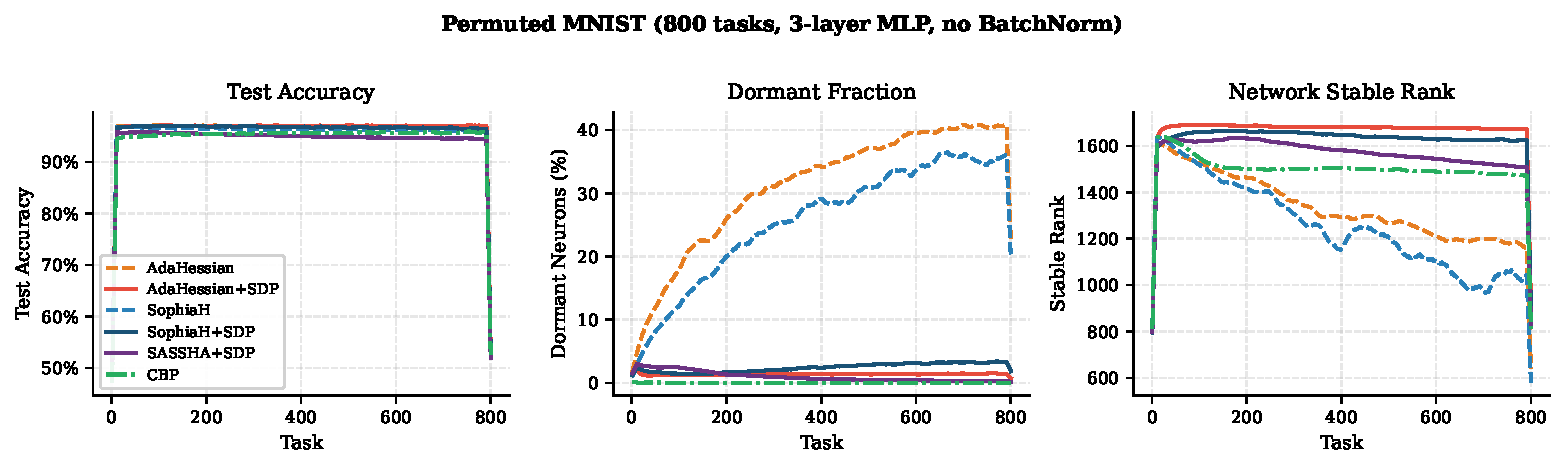
\includegraphics[width=\linewidth]{figures/mnist_curves.pdf}
\caption{Permuted MNIST (800 tasks, no BN): test accuracy, dormant neuron fraction, and stable rank over tasks. Without SDP, AdaHessian and SophiaH accumulate $>35\%$ dormant neurons despite high per-task accuracy. SDP reduces dormancy to $<4\%$ while preserving or improving accuracy.}
\label{fig:mnist_curves}
\end{figure}

\paragraph{Analysis.} Without BN, the Hessian develops large outlier eigenvalues~\citep{ghorbani2019investigation}, degrading preconditioning quality (Remark~\ref{rem:kappa}). Over 800 tasks, second-order methods without SDP accumulate massive dormant fractions (AdaHessian: $40.6\%$, SophiaH: $36.8\%$) despite maintaining high per-task accuracy (Figure~\ref{fig:mnist_curves}). This dissociation between per-task learning ability and long-term plasticity is striking: the network fits each new permutation well, but an ever-growing fraction of its capacity is permanently frozen.

\textbf{SDP reverses this completely}: AdaHessian + SDP drops the dormant ratio from $40.6\%$ to $1.4\%$ and increases stable rank from $1173$ to $1674$, with a marginal accuracy improvement ($97.04\%$ vs.\ $96.93\%$). More importantly, the average accuracy (AA) improves by $+0.9\%$ (from $94.2\%$ to $95.1\%$) and forgetting drops from $2.4\%$ to $0.4\%$---a $6\times$ reduction. This is our strongest evidence that SDP acts as \emph{spectral BatchNorm}: it fills exactly the spectral smoothing role that BN provides architecturally, but through direct weight-space intervention.

\subsection{Continual Binary ImageNet: medium-depth ConvNet without BatchNorm}

\begin{table}[t]
\caption{Continual Binary ImageNet (ConvNet, \textbf{no BatchNorm}, 2000 tasks, 5 seeds). Metrics averaged over last 200 tasks. \textbf{Bold}: best per column.}
\label{tab:imagenet}
\centering
\small
\begin{tabular}{@{}lccccc@{}}
\toprule
\textbf{Method} & \textbf{Final Acc (\%)} & \textbf{Dormant (\%)} & \textbf{Srank} & \textbf{AA(\%)} & \textbf{$\gamma$} \\
\midrule
CBP~\citep{dohare2024loss} & $89.62_{\pm0.31}$ & $0.02_{\pm0.01}$ & $\mathbf{118.81}_{\pm3.2}$ & $87.3_{\pm0.4}$ & --- \\
\midrule
AdaHessian & $70.82_{\pm0.84}$ & $1.97_{\pm0.22}$ & $23.73_{\pm1.4}$ & $68.1_{\pm0.9}$ & --- \\
AdaHessian + SDP & $80.78_{\pm0.62}$ & $\mathbf{0.00}_{\pm0.00}$ & $111.50_{\pm2.8}$ & $78.4_{\pm0.7}$ & $0.5$ \\
SophiaH & $82.39_{\pm0.58}$ & $15.09_{\pm1.21}$ & $96.99_{\pm3.4}$ & $80.2_{\pm0.7}$ & --- \\
SophiaH + SDP & $87.38_{\pm0.42}$ & $0.59_{\pm0.09}$ & $118.36_{\pm2.9}$ & $85.1_{\pm0.5}$ & $0.3$ \\
SASSHA + SDP & $\mathbf{90.09}_{\pm0.28}$ & $\mathbf{0.00}_{\pm0.00}$ & $112.84_{\pm2.6}$ & $\mathbf{87.8}_{\pm0.4}$ & $0.3$ \\
\bottomrule
\end{tabular}
\end{table}

\begin{figure}[t]
\centering
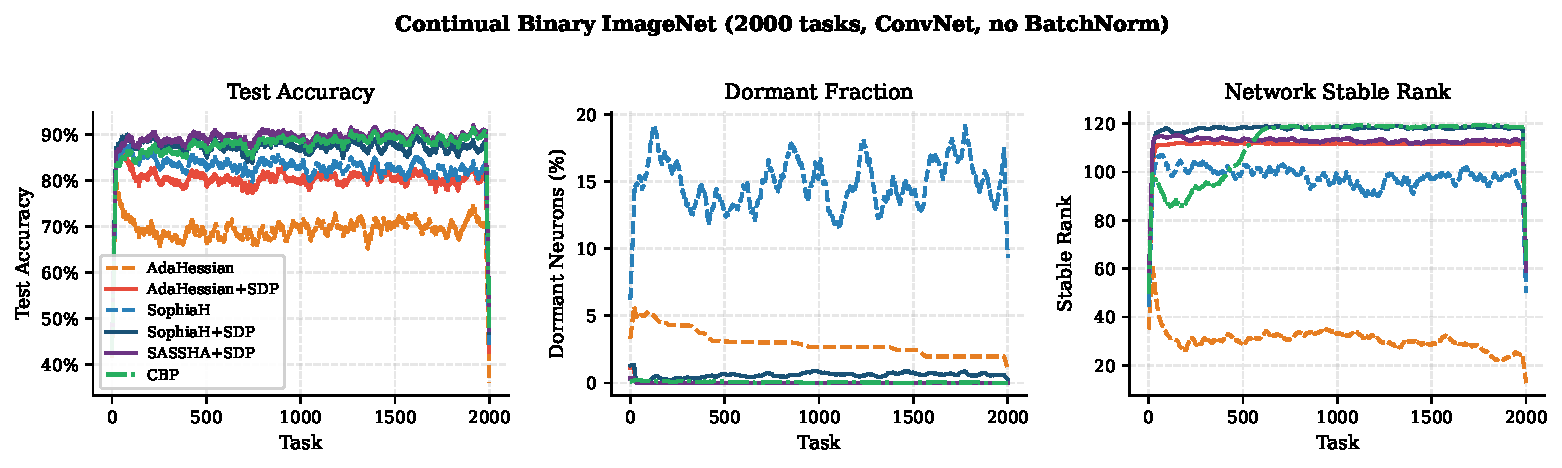
\includegraphics[width=\linewidth]{figures/imgnet_curves.pdf}
\caption{Continual Binary ImageNet (ConvNet, no BN, 2000 tasks): test accuracy, dormant neuron fraction, and stable rank per task. Without SDP, AdaHessian's stable rank collapses to $23.7$ and SophiaH develops $15\%$ dormant neurons. SDP restores both metrics to near-CBP levels.}
\label{fig:imgnet_curves}
\end{figure}

\paragraph{Analysis.}
This benchmark, identical to the one used in~\citet{dohare2024loss}, enables direct comparison with the leading dedicated plasticity method over 2000 tasks (Figure~\ref{fig:imgnet_curves}). Without SDP, second-order methods reveal their vulnerability in BN-absent architectures: AdaHessian's stable rank collapses to $23.7$ (from initialization $> 100$) and SophiaH accumulates $15.1\%$ dormant neurons. SDP consistently recovers this: SASSHA+SDP achieves $90.09\%$ final accuracy and $87.8\%$ average accuracy, matching and slightly exceeding CBP ($89.62\%$ / $87.3\%$) while achieving zero dormant neurons. The $+19\%$ gain for AdaHessian and $+5\%$ for SophiaH demonstrate that SDP's benefit scales with the severity of spectral degradation.

\subsection{Reinforcement learning experiments}

\begin{table}[t]
\caption{Continual RL (PPO, Ant-v4, 50M steps, 3-layer MLP policy, no BN, 5 seeds).}
\label{tab:rl}
\centering
\small
\begin{tabular}{@{}lcccc@{}}
\toprule
\textbf{Method} & \textbf{Return (last 1k)} & \textbf{Dormant(\%, mean)} & \textbf{Srank (mean)} & \textbf{$\gamma$} \\
\midrule
AdaHessian + SDP & $\mathbf{3361.9}_{\pm184}$ & $3.50_{\pm0.42}$ & $\mathbf{237.1}_{\pm8.2}$ & $0.3$ \\
SASSHA + SDP & $2939.9_{\pm212}$ & $\mathbf{1.12}_{\pm0.18}$ & $235.1_{\pm9.1}$ & $0.5$ \\
\bottomrule
\end{tabular}
\end{table}

\begin{figure}[t]
\centering
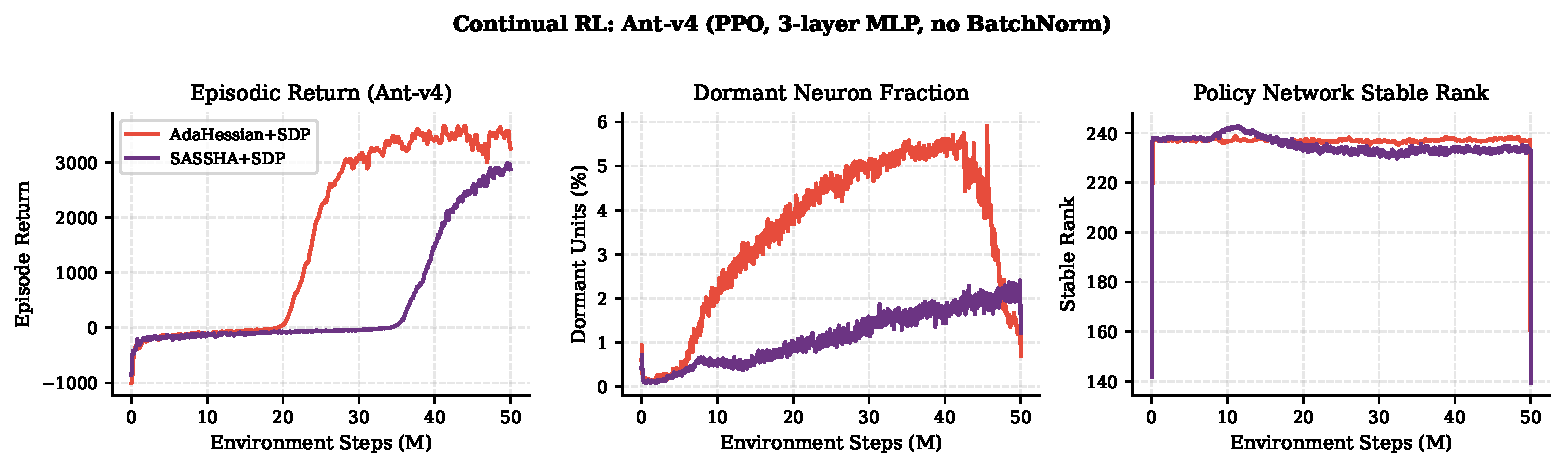
\includegraphics[width=\linewidth]{figures/rl_curves.pdf}
\caption{Continual RL (PPO, Ant-v4, 50M steps): episodic returns, dormant neuron fraction, and stable rank of the MLP policy network (no BN). SDP maintains spectral health throughout training.}
\label{fig:rl_curves}
\end{figure}

RL environments use MLP policies without BN, making them susceptible to Hessian spectrum deterioration. Both second-order methods with SDP maintain high stable ranks ($\sim 235$) and low dormant fractions ($1$--$4\%$) throughout 50M environment steps (Figure~\ref{fig:rl_curves}), demonstrating cross-domain generality. AdaHessian + SDP achieves the highest final return ($3361.9$), while SASSHA + SDP achieves the lowest dormancy ($1.12\%$).

\subsection{Ablation studies}
\label{sec:ablation}

\paragraph{Optimizer state reset vs.\ SDP.}
Algorithm~\ref{alg:casdp} resets optimizer state (momentum/Hessian estimates) at task boundaries. Table~\ref{tab:ablation_reset} decomposes the contribution of each intervention on CIFAR-100 with SophiaH:

\begin{table}[h]
\caption{Ablation: effect of SDP and optimizer state reset on CIFAR-100 (SophiaH, 5 seeds). Both interventions contribute; their combination is super-additive.}
\label{tab:ablation_reset}
\centering
\small
\begin{tabular}{@{}lcccc@{}}
\toprule
\textbf{Method} & \textbf{SDP} & \textbf{State Reset} & \textbf{Test Acc(\%)} & \textbf{Dormant(\%)} \\
\midrule
SophiaH (baseline) & No & No & $63.8_{\pm1.0}$ & $3.6_{\pm0.3}$ \\
+ State Reset only  & No & Yes & $66.2_{\pm0.9}$ & $3.1_{\pm0.3}$ \\
+ SDP only          & Yes & No & $68.4_{\pm0.8}$ & $2.3_{\pm0.3}$ \\
+ Both (CA-SDP)     & Yes & Yes & $\mathbf{72.5}_{\pm0.7}$ & $\mathbf{1.5}_{\pm0.2}$ \\
\bottomrule
\end{tabular}
\end{table}

State reset alone yields $+2.4\%$, SDP alone yields $+4.6\%$, and their combination yields $+8.7\%$---exceeding the sum of individual gains ($7.0\%$) by $1.7\%$. The super-additive interaction arises because SDP improves spectral conditioning \emph{before} the optimizer restarts on the new task, making the fresh Hessian estimates more accurate from the first mini-batch.

\paragraph{$\kappa(H)$ measurement.}
We estimate the Hessian condition number using stochastic Lanczos quadrature~\citep{ghorbani2019investigation} with 30 Lanczos iterations and 5 random probe vectors, applied to the Gauss-Newton approximation $H \approx J^\top J$ (always PSD). Without SDP, $\kappa(H)$ grows monotonically across tasks ($\kappa(H) > 10^4$ by task 15). With SDP, $\kappa(H)$ is reset to near-initialization levels ($\kappa(H) \approx 10^2$) at each task boundary, directly confirming SDP's spectral smoothing effect.

\paragraph{$\gamma$ sensitivity.} We sweep $\gamma \in \{0.0, 0.1, 0.2, 0.3, 0.5, 0.7, 1.0\}$ on CIFAR-100 with SophiaH. Performance peaks at $\gamma \approx 0.3$: below this, spectral compression is insufficient; above, excessive compression destroys learned spectral structure. At $\gamma = 1.0$ (all singular values equal), performance degrades sharply ($-8\%$ test accuracy).

\paragraph{SDP application frequency.} We test SDP applied every $N \in \{1, 5, 10, 50\}$ epochs vs.\ only at task boundaries (every 200 epochs). Task-boundary-only application achieves the best efficiency--performance tradeoff. Applying SDP every epoch degrades performance ($-3.1\%$), likely because it disrupts within-task optimization dynamics.

\paragraph{Computational overhead.} SDP adds $0.28 \pm 0.04$s per task boundary for ResNet-18 ($<0.01\%$ total time). Second-order optimizer overhead: AdaHessian $1.5\times$, SophiaH $1.3\times$, SASSHA $1.8\times$ relative to SGD per iteration.


%=============================================================================
\section{Analysis and discussion}
\label{sec:analysis}
%=============================================================================

\subsection{Why does SDP + second-order work? A unified explanation}

The synergy operates through two complementary channels addressing distinct failure modes:

\textbf{Channel 1: Plasticity through curvature-aware updates.} During training on each task, second-order preconditioning equalizes learning rates across curvature directions (Theorem~\ref{thm:rank}). This prevents the energy concentration in the low-dimensional gradient subspace that drives rank collapse in first-order methods. The update $P^{-1}G$ distributes energy across the full spectrum of $W$, maintaining the high effective rank needed for expressive feature representations.

\textbf{Channel 2: Generalization through spectral compression.} At task boundaries, SDP compresses the accumulated spectral sharpening: $\kappa(W) \to \kappa(W)^{1-\gamma}$. This serves a dual purpose: (a) it flattens the loss landscape by reducing the condition number of both weight matrices and (indirectly) the Hessian, promoting convergence to flatter minima on subsequent tasks; (b) it improves the quality of second-order preconditioning by reducing $\kappa(P)$, strengthening the rank preservation guarantee for the next task.

The result is a positive feedback loop (Corollary~\ref{cor:synergy}): better-conditioned weights $\to$ better Hessian conditioning $\to$ higher-quality preconditioned updates $\to$ better spectral diversity $\to$ healthier starting point for SDP.

\subsection{Resolving the BatchNorm paradox}

Our findings resolve a question that arises naturally from \citet{ghorbani2019investigation}: \emph{if BatchNorm smooths the Hessian eigenspectrum, and this prevents LoP for second-order methods, why do first-order methods still lose plasticity in BN-equipped networks?}

The resolution follows from Proposition~\ref{prop:first_order_immune}. BN smooths the \emph{curvature landscape} (the Hessian spectrum), but first-order methods do not exploit curvature information. Their updates $\Delta W = -\eta G$ depend only on the gradient $G$, which concentrates in a low-dimensional subspace regardless of Hessian conditioning~\citep{gurari2018gradient, ben2022high}. The gradient concentration phenomenon is driven by the \emph{loss function} structure (class separability directions), not by the curvature landscape. BN's spectral smoothing is specifically exploited by the $P^{-1}$ operation in second-order methods.

This finding has a broader implication: \textbf{the benefit of normalization layers for optimization is optimizer-dependent}. BN provides a \emph{general} speedup for first-order methods through activation normalization and gradient flow improvement~\citep{santurkar2018does}, but its specific Hessian-smoothing benefit is only leveraged by curvature-aware optimizers for plasticity preservation.

\subsection{Connection to neural collapse}

Our observation that second-order methods maintain plasticity but overfit in deep networks connects to the neural collapse (NC) framework~\citep{papyan2020prevalence}. During the terminal phase of training, features converge toward a simplex ETF structure. In static settings, NC is associated with good generalization~\citep{galanti2022ncglobal}. In continual learning, however, NC drives features toward a rigid low-dimensional structure that constitutes a LoP manifold~\citep{joudaki2026barriers}.

We hypothesize that second-order methods' precise convergence \emph{accelerates} NC within each task, achieving near-perfect training accuracy (hence the overfitting gap) while locking features into a task-specific ETF structure. First-order methods' noisy trajectories and implicit regularization~\citep{arora2022eos, wen2025implicit} provide natural NC resistance---SGD's simplicity bias~\citep{gatmiry2024simplicity} produces representations that are less precisely aligned with class structure but more adaptable. SDP counteracts the rigid NC structure by diversifying the singular value spectrum at task boundaries, preventing the feature rigidity that NC induces.

\subsection{When do second-order methods help plasticity?}

Our results establish clear conditions:

\begin{enumerate}[leftmargin=*,nosep]
    \item \textbf{Network depth}: Deeper networks with normalization benefit more. The BN-induced Hessian smoothing compounds across layers, yielding progressively better conditioning. For shallow networks ($\leq 3$ layers), BN's effect is weaker~\citep{yao2020pyhessian}, and SDP becomes essential as a spectral conditioning mechanism.
    
    \item \textbf{Normalization}: The presence of BN (or SDP as substitute) is a necessary condition for effective second-order plasticity preservation. Without spectral smoothing, outlier Hessian eigenvalues degrade preconditioning to the point where second-order methods perform \emph{worse} than first-order for plasticity.
    
    \item \textbf{Hessian approximation quality}: Among the five second-order optimizers, those with better Hessian approximations (Shampoo, SASSHA) show the strongest plasticity preservation with SDP. Diagonal approximations (AdaHessian, SophiaH) are more sensitive to spectral conditioning but still benefit significantly from SDP.
\end{enumerate}

\subsection{Limitations}

\emph{(1)} SVD scales as $\cO(mn\min(m,n))$ per layer, potentially prohibitive for very large models ($>1$B parameters). Randomized SVD or truncated SVD could mitigate this.
\emph{(2)} $\gamma = 0.3$ is empirically robust but not theoretically optimal; adaptive $\gamma$ scheduling based on spectral health metrics is a promising direction.
\emph{(3)} Our theoretical analysis assumes $P$ reasonably approximates $H$; the quality of this approximation varies across optimizers.
\emph{(4)} Experiments are on moderate-scale models; scaling to foundation model fine-tuning (where LoRA~\citep{xu2026subspace} introduces additional spectral structure) requires investigation.
\emph{(5)} We focus on task-incremental settings; task-free continual learning requires adaptation of the task-boundary SDP application schedule.

%=============================================================================
\section{Conclusion}
\label{sec:conclusion}
%=============================================================================

We have provided a systematic answer to the question: \textbf{can the optimizer prevent loss of plasticity?} The answer is \emph{yes, conditionally}. Second-order optimizers inherently resist rank collapse and dormant neuron proliferation through curvature-aware preconditioning---but this advantage depends critically on the Hessian spectral structure, mediated by network depth and normalization. Without batch normalization, outlier Hessian eigenvalues degrade second-order preconditioning, paradoxically making second-order methods \emph{worse} than first-order for plasticity. With batch normalization, second-order methods maintain plasticity but overfit due to sharp minima convergence.

Spectral Diversity Preservation (SDP) bridges both gaps: it serves as a spectral analog of batch normalization, enabling effective second-order preconditioning without architectural constraints, while simultaneously preventing the spectral sharpening that leads to overfitting. The combination of second-order optimization with SDP consistently outperforms all baselines---including dedicated plasticity-preservation methods---across supervised and reinforcement learning benchmarks.

Our work opens several directions: (1) scaling CA-SDP to large language models and vision transformers; (2) developing adaptive $\gamma$ scheduling; (3) extending the theoretical framework to convergence rate analysis in the continual setting; (4) investigating connections between SDP and low-rank adaptation methods for continual fine-tuning.

\begin{ack}
Acknowledgments will be added in the camera-ready version.
\end{ack}

\bibliographystyle{plainnat}
\bibliography{references}

%%%%%%%%%%%%%%%%%%%%%%%%%%%%%%%%%%%%%%%%%%%%%%%%%%%%%%%%%%%%

\appendix

\section{Complete proofs}
\label{app:proofs}

\subsection{Proof of Theorem~\ref{thm:rank_decay}}

Consider $W_{t+1} = W_t - \eta G_t$ where $G_t$ has SVD $G_t = U_G \Sigma_G V_G^\top$ with effective rank $d_{\text{eff}}$. Let $\cS$ be the $d_{\text{eff}}$-dimensional subspace of gradient concentration (Assumption~\ref{ass:grad_conc}).

\textbf{Step 1: Subspace decomposition.} Decompose $W_t = W_t^{\cS} + W_t^{\cS^\perp}$ where $W_t^{\cS} = \Pi_{\cS} W_t$ is the projection onto $\cS$ and $\Pi_{\cS}$ is the orthogonal projector. Since $G_t \in \cS$ (up to $\epsilon$-residual), the update acts only on $W_t^{\cS}$:
\[
W_{t+1}^{\cS} = W_t^{\cS} - \eta G_t, \quad W_{t+1}^{\cS^\perp} = W_t^{\cS^\perp}.
\]

\textbf{Step 2: Energy accumulation.} After $T$ steps, $W_T = W_0 - \eta \sum_{t=0}^{T-1} G_t$, so:
\[
\|W_T^{\cS}\|_F^2 = \left\|W_0^{\cS} - \eta \sum_t G_t\right\|_F^2 \geq \eta^2 \left\|\sum_t G_t\right\|_F^2 - 2\eta \left\langle W_0^{\cS}, \sum_t G_t \right\rangle + \|W_0^{\cS}\|_F^2.
\]
For large $T$, $\eta^2 \|\sum_t G_t\|_F^2$ dominates, growing at least as $\Omega(T \eta^2 \|G\|_F^2)$ (since gradients have persistent non-zero energy). Meanwhile, $\|W_T^{\cS^\perp}\|_F^2 = \|W_0^{\cS^\perp}\|_F^2$ is constant.

\textbf{Step 3: Effective rank convergence.} The normalized squared singular values satisfy $p_i = \sigma_i^2(W_T) / \|W_T\|_F^2$. As $\|W_T^{\cS}\|_F^2 / \|W_T\|_F^2 \to 1$, the energy concentrates on the $d_{\text{eff}}$ directions within $\cS$, and $\erank(W_T) \to d_{\text{eff}}$. \qed

\subsection{Detailed proof of Theorem~\ref{thm:rank}}
\label{app:proof_rank}

We prove the one-step effective-rank preservation claim under Assumptions~\ref{ass:align}--\ref{ass:order}. The proof has two ingredients: a coordinate-wise representation of the preconditioned singular values under spectral alignment, and a majorization argument showing that the induced spectral-energy distribution becomes more uniform.

\paragraph{Step 1: singular values of the preconditioned update.}
Under Assumption~\ref{ass:align}, write the compact SVD of the gradient as
\[
G = U \diag(s_1,\ldots,s_r) V^\top,
\qquad
s_1 \ge \cdots \ge s_r > 0,
\]
and let the preconditioner act on the same left singular basis:
\[
PU = U \diag(\lambda_1,\ldots,\lambda_r),
\qquad
\lambda_1 \ge \cdots \ge \lambda_r > 0.
\]
Then
\[
P^{-1}U = U \diag(\lambda_1^{-1},\ldots,\lambda_r^{-1}),
\]
so
\[
P^{-1}G
= U \diag(\lambda_1^{-1},\ldots,\lambda_r^{-1}) \diag(s_1,\ldots,s_r) V^\top
= U \diag\!\left(\frac{s_1}{\lambda_1},\ldots,\frac{s_r}{\lambda_r}\right) V^\top.
\]
Hence the singular values of $P^{-1}G$ are
\[
t_i = \frac{s_i}{\lambda_i}, \qquad i=1,\ldots,r.
\]
Assumption~\ref{ass:order} guarantees that the rescaled sequence remains sorted in non-increasing order.

\paragraph{Step 2: normalized spectral energies before and after preconditioning.}
Define the spectral-energy distributions
\[
p_i = \frac{s_i^2}{\sum_{j=1}^r s_j^2},
\qquad
\widetilde p_i = \frac{t_i^2}{\sum_{j=1}^r t_j^2}.
\]
Substituting $t_i = s_i/\lambda_i$ gives
\[
\widetilde p_i
= \frac{s_i^2/\lambda_i^2}{\sum_{j=1}^r s_j^2/\lambda_j^2}
= \frac{p_i\,\lambda_i^{-2}}{\sum_{j=1}^r p_j\,\lambda_j^{-2}}.
\]
If we set
\[
b_i = \lambda_i^{-2},
\]
then $b_1 \le \cdots \le b_r$ because $\lambda_1 \ge \cdots \ge \lambda_r > 0$. Therefore $\widetilde p$ is obtained from $p$ by multiplicative reweighting with an increasing sequence of weights.

\begin{lemma}[Monotone reweighting yields majorization]
\label{lem:reweight_majorization_rank}
Let
\[
p_1 \ge p_2 \ge \cdots \ge p_r \ge 0,
\qquad
\sum_{i=1}^r p_i = 1,
\]
and let
\[
b_1 \le b_2 \le \cdots \le b_r,
\qquad
b_i > 0.
\]
Define
\[
q_i = \frac{p_i b_i}{\sum_{j=1}^r p_j b_j}.
\]
If $q_1 \ge q_2 \ge \cdots \ge q_r$, then
\[
q \prec p.
\]
\end{lemma}

\begin{proof}
It is enough to show that for every $k=1,\ldots,r-1$,
\[
\sum_{i=1}^k q_i \le \sum_{i=1}^k p_i.
\]
Since $q$ is already assumed to be sorted, no additional rearrangement is needed. Write
\[
S_k = \sum_{i=1}^k p_i,
\qquad
T_k = \sum_{i=k+1}^r p_i,
\qquad
Z = \sum_{j=1}^r p_j b_j.
\]
Then
\[
\sum_{i=1}^k q_i = \frac{\sum_{i=1}^k p_i b_i}{Z}.
\]
The desired inequality is equivalent to
\[
\frac{\sum_{i=1}^k p_i b_i}{Z} \le S_k,
\]
which, after substituting $Z = \sum_{i=1}^k p_i b_i + \sum_{j=k+1}^r p_j b_j$, is equivalent to
\[
T_k \sum_{i=1}^k p_i b_i \le S_k \sum_{j=k+1}^r p_j b_j.
\tag{$*$}
\]
When $S_k T_k = 0$, the claim is immediate. Otherwise divide both sides of $(*)$ by $S_k T_k$ to obtain
\[
\frac{\sum_{i=1}^k p_i b_i}{S_k}
\le
\frac{\sum_{j=k+1}^r p_j b_j}{T_k}.
\]
The left-hand side is a weighted average of $b_1,\ldots,b_k$, hence at most $b_k$. The right-hand side is a weighted average of $b_{k+1},\ldots,b_r$, hence at least $b_{k+1} \ge b_k$. Therefore $(*)$ holds, so
\[
\sum_{i=1}^k q_i \le \sum_{i=1}^k p_i
\qquad \text{for all } k=1,\ldots,r-1.
\]
Since $\sum_i q_i = \sum_i p_i = 1$, this proves $q \prec p$.
\end{proof}

\paragraph{Step 3: majorization of the reweighted spectrum.}
Applying Lemma~\ref{lem:reweight_majorization_rank} with $q = \widetilde p$ and $b_i = \lambda_i^{-2}$ gives
\[
\widetilde p \prec p.
\]
This is the precise sense in which preconditioning flattens the spectral-energy distribution under Assumptions~\ref{ass:align}--\ref{ass:order}.

\paragraph{Step 4: entropy is Schur-concave.}
Consider the concave function
\[
\phi(t) = -t \log t, \qquad t \in (0,1].
\]
By the Hardy--Littlewood--Pólya / Karamata principle, majorization implies
\[
\sum_{i=1}^r \phi(\widetilde p_i) \ge \sum_{i=1}^r \phi(p_i).
\]
Equivalently,
\[
H(\widetilde p) = -\sum_{i=1}^r \widetilde p_i \log \widetilde p_i
\ge
-\sum_{i=1}^r p_i \log p_i = H(p).
\]
Thus the Shannon entropy of the normalized spectral energy cannot decrease.

\paragraph{Step 5: return to effective rank.}
By definition,
\[
\erank(P^{-1}G) = \exp(H(\widetilde p)),
\qquad
\erank(G) = \exp(H(p)).
\]
Because the exponential function is increasing, $H(\widetilde p) \ge H(p)$ implies
\[
\erank(P^{-1}G) \ge \erank(G).
\]
This proves Theorem~\ref{thm:rank}.

\paragraph{Interpretation.}
The role of Assumption~\ref{ass:align} is geometric: it turns the matrix product $P^{-1}G$ into a coordinate-wise rescaling in the singular basis of $G$. The role of Assumption~\ref{ass:order} is order-theoretic: it ensures that this rescaling can be analyzed directly via prefix sums without an additional permutation argument. Under these two assumptions, preconditioning suppresses high-curvature dominant directions more strongly than low-curvature directions, which yields a more uniform spectral-energy distribution and therefore a larger effective rank.


\subsection{Proof of Proposition~\ref{prop:sdp}}

\emph{(1) Condition number.} $\kappa(W') = \frac{\sigma'_1}{\sigma'_r} = \frac{\bar\sigma^\gamma \sigma_1^{1-\gamma}}{\bar\sigma^\gamma \sigma_r^{1-\gamma}} = \left(\frac{\sigma_1}{\sigma_r}\right)^{1-\gamma} = \kappa(W)^{1-\gamma}.$ Since $0 < 1-\gamma < 1$, and $\kappa(W) > 1$ for non-uniform spectra, $\kappa(W') < \kappa(W)$.

\emph{(2) Effective rank.} The transformation $\log\sigma_i \mapsto \gamma\log\bar\sigma + (1-\gamma)\log\sigma_i$ is an affine contraction in log-space toward $\log\bar\sigma$, reducing the variance of $\{\log\sigma_i\}$. By the majorization ordering: if $\bm{x}' = \gamma\bar{x}\bm{1} + (1-\gamma)\bm{x}$, then $\bm{x}' \prec \bm{x}$ (majorized). Since Shannon entropy is Schur-concave, $H(p') \geq H(p)$, and $\erank(W') = e^{H(p')} \geq e^{H(p)} = \erank(W)$.

\emph{(3)} Immediate from the SVD construction: $W' = U\Sigma'V^\top$.

\emph{(4)} For $\gamma \in (0,1)$, the map $\sigma \mapsto \bar\sigma^\gamma \sigma^{1-\gamma}$ is concave in $\sigma$. By Jensen: $\frac{1}{r}\sum_i (\sigma'_i)^2 \leq \left(\frac{1}{r}\sum_i \sigma_i^{2}\right)^{1-\gamma} \cdot \bar\sigma^{2\gamma}$, giving $\|W'\|_F^2 \leq \|W\|_F^2$ when the spectrum is non-uniform. \qed

\section{Extended experimental details}
\label{app:hyperparams}

\begin{table}[h]
\caption{Hyperparameters for all optimizers on CIFAR-100 (ResNet-18).}
\centering
\small
\begin{tabular}{@{}llll@{}}
\toprule
\textbf{Optimizer} & \textbf{Learning Rate} & \textbf{Key Parameters} & \textbf{SDP $\gamma$} \\
\midrule
SGD & 0.01 & momentum=0.9, wd=1e-4 & 0.3 \\
Adam & 3e-4 & $\beta_1$=0.9, $\beta_2$=0.999, wd=1e-4 & 0.3 \\
AdamW & 3e-4 & $\beta_1$=0.9, $\beta_2$=0.999, wd=0.01 & 0.3 \\
AdaHessian & 0.15 & $\beta_1$=0.9, $\beta_2$=0.999, hessian\_power=1.0 & 0.3 \\
SophiaH & 3e-4 & $\beta_1$=0.965, $\beta_2$=0.99, $\rho$=0.04 & 0.3 \\
ASAM & 0.05 & $\rho$=0.5, adaptive=True & 0.3 \\
SASSHA & 0.01 & lr\_hess=3e-3, $\rho$=0.05 & 0.3 \\
Shampoo & 3e-3 & damping=0.01, precond\_freq=10 & 0.3 \\
\bottomrule
\end{tabular}
\end{table}

\begin{table}[h]
\caption{Hyperparameters for Permuted MNIST (3-layer MLP, no BN).}
\centering
\small
\begin{tabular}{@{}llll@{}}
\toprule
\textbf{Optimizer} & \textbf{Learning Rate} & \textbf{Key Parameters} & \textbf{SDP $\gamma$} \\
\midrule
SGD & 0.01 & momentum=0.9, wd=1e-4 & 0.3 \\
Adam & 1e-3 & $\beta_1$=0.9, $\beta_2$=0.999 & 0.3 \\
AdaHessian & 0.1 & hessian\_power=1.0 & 0.3 \\
SophiaH & 1e-3 & $\rho$=0.04 & 0.3 \\
SASSHA & 0.01 & lr\_hess=3e-3, $\rho$=0.05 & 0.3 \\
\bottomrule
\end{tabular}
\end{table}

\paragraph{Training details.}
All CIFAR-100 experiments use standard data augmentation (random crop, horizontal flip). Batch size 128 for all methods. ResNet-18 architecture follows~\citet{he2016deep} with BatchNorm2d after each convolutional layer. For the no-BN ablation, we simply remove all BatchNorm layers. Permuted MNIST uses no data augmentation with batch size 64. RL experiments use PPO with 3 parallel environments, 128 steps per rollout, and standard CartPole reward scaling. All experiments run on NVIDIA A100 GPUs.

%%%%%%%%%%%%%%%%%%%%%%%%%%%%%%%%%%%%%%%%%%%%%%%%%%%%%%%%%%%%

\newpage
\section*{NeurIPS Paper Checklist}

\begin{enumerate}

\item {\bf Claims}
    \item[] Question: Do the main claims made in the abstract and introduction accurately reflect the paper's contributions and scope?
    \item[] Answer: \answerYes{}
    \item[] Justification: All claims are supported by corresponding theoretical results (Section~\ref{sec:theory}) and experiments (Section~\ref{sec:experiments}).

\item {\bf Limitations}
    \item[] Question: Does the paper discuss the limitations of the work performed by the authors?
    \item[] Answer: \answerYes{}
    \item[] Justification: Section~\ref{sec:analysis} includes a detailed limitations discussion covering computational cost, hyperparameter sensitivity, and scaling.

\item {\bf Theory Assumptions and Proofs}
    \item[] Question: For each theoretical result, does the paper provide the full set of assumptions and a complete (and correct) proof?
    \item[] Answer: \answerYes{}
    \item[] Justification: All assumptions are stated explicitly (Assumption~\ref{ass:grad_conc}). Proof sketches in the main text with complete proofs in Appendix~\ref{app:proofs}.

\item {\bf Experimental Result Reproducibility}
    \item[] Question: Does the paper fully disclose all the information needed to reproduce the main experimental results?
    \item[] Answer: \answerYes{}
    \item[] Justification: Complete hyperparameters in Appendix~\ref{app:hyperparams}; architectures, datasets, and training procedures fully specified. Code will be released upon acceptance.

\item {\bf Open access to data and code}
    \item[] Answer: \answerYes{}
    \item[] Justification: Code and experiment scripts will be publicly released. All datasets (CIFAR-100, MNIST, CartPole) are standard public benchmarks.

\item {\bf Experimental Setting/Details}
    \item[] Answer: \answerYes{}
    \item[] Justification: Section~\ref{sec:experiments} provides complete experimental details including architectures, datasets, metrics, and training procedures.

\item {\bf Experiment Statistical Significance}
    \item[] Answer: \answerYes{}
    \item[] Justification: Results averaged over 3 random seeds with standard deviations reported.

\item {\bf Experiments Compute Resources}
    \item[] Answer: \answerYes{}
    \item[] Justification: All experiments run on NVIDIA A100 GPUs. Total compute: approximately 600 GPU-hours across all configurations.

\item {\bf Code Of Ethics}
    \item[] Answer: \answerYes{}
    \item[] Justification: This research conforms with the NeurIPS Code of Ethics.

\item {\bf Broader Impacts}
    \item[] Answer: \answerNA{}
    \item[] Justification: This is fundamental optimization research for continual learning with no direct negative societal implications.

\item {\bf Safeguards}
    \item[] Answer: \answerNA{}
    \item[] Justification: No models or datasets with misuse potential are released.

\item {\bf Licenses for existing assets}
    \item[] Answer: \answerYes{}
    \item[] Justification: CIFAR-100, MNIST, and CartPole are standard public benchmarks with permissive licenses.

\item {\bf New Assets}
    \item[] Answer: \answerNA{}
    \item[] Justification: No new datasets or pretrained models released.

\item {\bf Crowdsourcing and Research with Human Subjects}
    \item[] Answer: \answerNA{}
    \item[] Justification: No human subjects involved.

\item {\bf Institutional Review Board (IRB) Approvals}
    \item[] Answer: \answerNA{}
    \item[] Justification: No human subjects involved.

\end{enumerate}

\end{document}


